\documentclass[xcolor=svgnames]{beamer}
\usepackage[utf8x]{inputenc}
%\usepackage[spanish]{babel}
\usepackage{times}
\usepackage{cite}
\usepackage{xcolor}
\usepackage{multicol}
\usepackage{url}
\usepackage{alltt}
\usepackage{amsthm}
\usepackage{color}
\usepackage{CJK}
\usepackage{enumerate}
\usepackage{listings}
\usepackage{textpos}
\usepackage{fancybox}
\usepackage{eurosym}
\usepackage{graphics,graphicx,color,colortbl}
\usepackage{subfigure}
\usepackage{algorithm}
\usepackage{float}
\usepackage{graphicx}
%\usepackage{subcaption}
\usepackage{subfloat}

\usetheme{Berlin}
\useoutertheme{shadow}
\useoutertheme{split}
\useinnertheme{rounded}
\useoutertheme{infolines}
\usecolortheme{orchid}
\usecolortheme{whale}
\setbeamertemplate{navigation symbols}{}
\setbeamercolor{bgcolor}{fg=black,bg=GhostWhite}
\setbeamercovered{transparent}

\title{Volcanic Environments}
\subtitle{Robots for Exploration and Measurement}
\author[David Martínez y Luis Melo]{David Ricardo Martínez Hernández \\ Luis Aníbal Melo Rivera}
\institute[UNAL]{Faculty of Engineer\\ Department of Electric and Electronic \\ National University Of Colombia}
\date[08/27/2012]{August $27$, $2012$}

\begin{document}
\begin{frame}
\titlepage
\end{frame}

\begin{frame}
\tableofcontents
\end{frame}

\section{Introduction}
\begin{frame}
  \frametitle{Introduction}
    \begin{itemize}
   \item The study of volcanic activity is important from a scientific point of view as it allows for a better understanding of one of the most spectacular geological phenomena and of the working principles that are at the basis of geophysics. \pause
   \item Most of the measurements necessary for a comprehensive analysis of what is taking place inside a volcano should be taken in the proximity of the craters. \pause
   \item The knowledge of when and how a plume of volcanic ash will be emitted is useful for the advanced planning of route modifications, and if need be, flight cancellations; thereby, this information can help reduce inconvenience and discomfort to passengers.
  \end{itemize}
\end{frame}

\section{Importance of Robots for Measurements in Volcanoes}
\begin{frame}
\frametitle{Importance of Robots for Measurements in Volcanoes}
  \begin{itemize}
   \item Reduce the level of risk involved for volcanologists who are working too closely to volcanic vents during eruptive phenomena.\pause
   \item Measurement of variables relevant to the investigation of volcanic activity (visual, thermal images, gas analysis and sampling). \pause
   \item Several environmental constraints must be taken into account in the developmental phase of a robotic system that is to be adopted in volcanic areas (Terrain, Temperatures, Gases, and Weather Conditions).
  \end{itemize}
\end{frame}

\section{Other projects concerning Robots and Volcanoes}
\begin{frame}
 \frametitle{Other projects concerning Robots and Volcanoes}
    \begin{figure}
      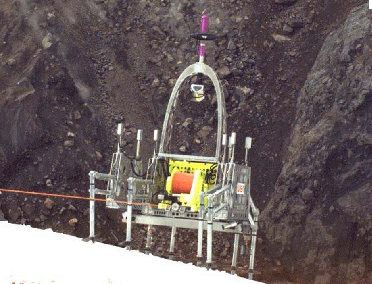
\includegraphics[scale=0.55]{1.png}
	\caption{Dante II\footnote{Copy  of \url{http://syahbta.blogspot.com/2010/10/4-kandidat-pengganti-mbah-marijan.html}}}
    \end{figure}
\end{frame}

\begin{frame}
    \begin{figure}
      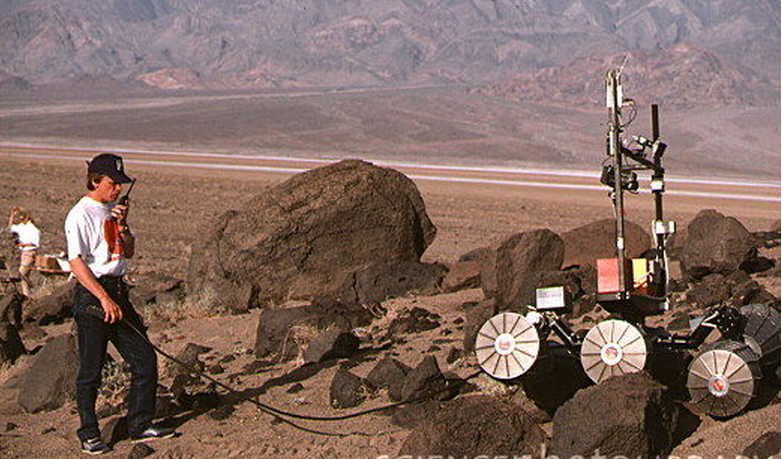
\includegraphics[scale=0.40]{2.png}
	\caption{Rover Marsokhod\footnote{Copy  of \url{http://www.sciencephoto.com/media/337613/enlarge}}}
    \end{figure}
\end{frame}

\begin{frame}
    \begin{figure}
      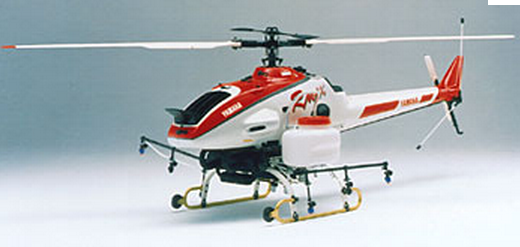
\includegraphics[scale=0.60]{3.png}
	\caption{Yamaha RMAX\footnote{Copy  of \url{http://www.yamaha-motor.co.jp/global/news/2002/02/06/sky.html}}}
    \end{figure}
\end{frame}

\begin{frame}
    \begin{figure}
      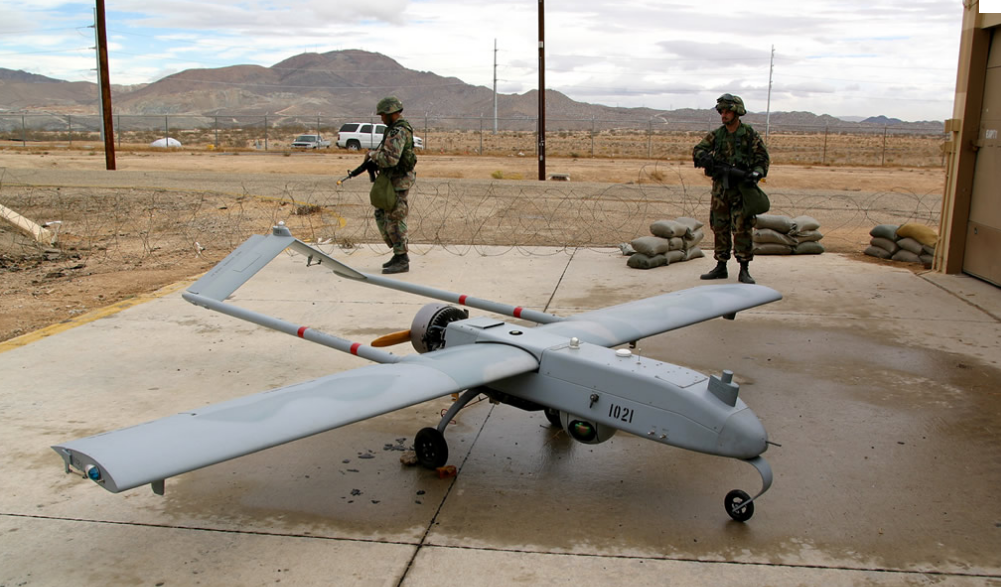
\includegraphics[scale=0.30]{4.png}
	\caption{UAV Makers AAI \& Aerosonde\footnote{Copy  of \url{http://www.defenseindustrydaily.com/textron-buys-uav-makers-aai-aerosonde-03968/}}}
    \end{figure}
\end{frame}

\begin{frame}
    \begin{figure}
      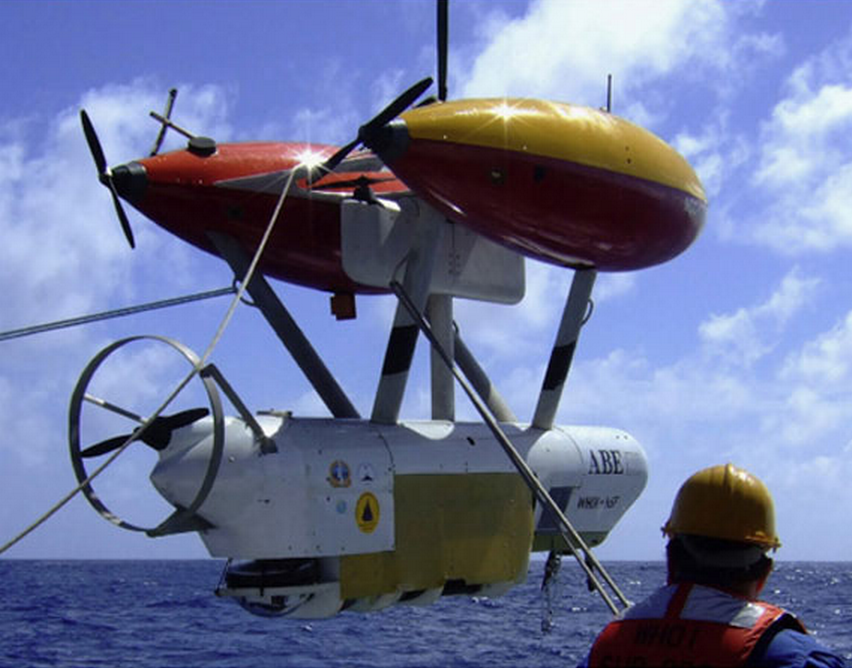
\includegraphics[scale=0.250]{5.png}
	\caption{Autonomous Benthic Explorer (ABE)\footnote{Copy  of \url{http://oceanexplorer.noaa.gov/explorations/10chile/background/plan/media/missionplan3_es.html}}}
    \end{figure}
\end{frame}

\begin{frame}
    \begin{figure}
      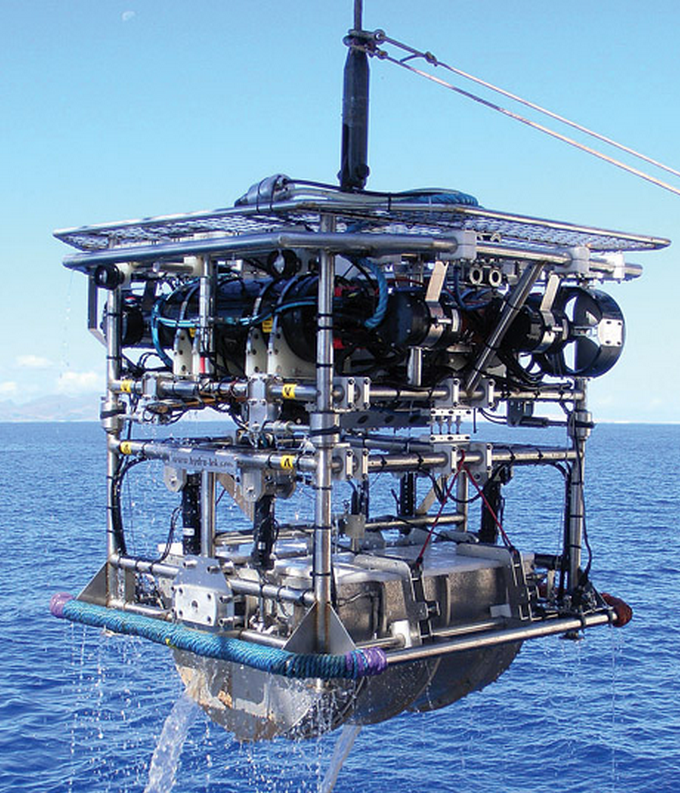
\includegraphics[scale=0.2350]{6.png}
	\caption{HyBIS\footnote{Copy  of \url{http://www.intoceansys.co.uk/articles-detail.php}}}
    \end{figure}
\end{frame}

\section{ROBOVOLC}
\subsection{Prototype Robots}
\begin{frame}
\frametitle{Prototype Robots}
    \begin{figure}[H]
	\centering
      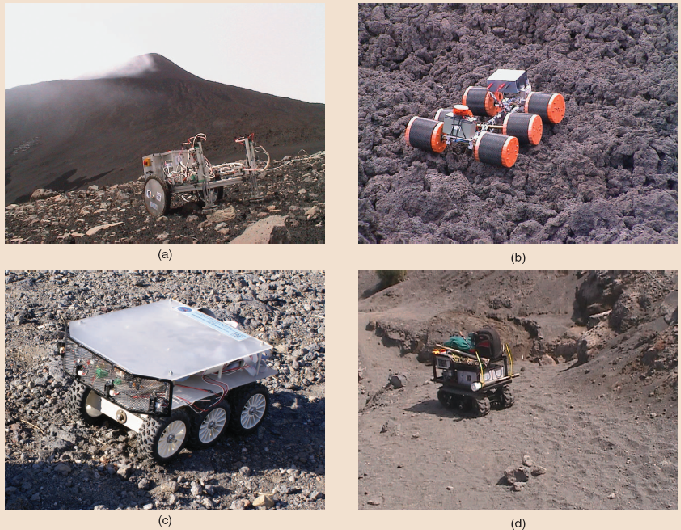
\includegraphics[scale=0.31]{7.png}
	\caption{{\scriptsize (a) Wheeleg in action, (b) M6 on volcanic terrain, (c) P6W robot, (d) U-Go robot\footnote{Image copy of ``\textit{IEEE Robotics And Automation Society}'', Volume $19$ No. $1$ March $2012$ ISSN $1070-9932$ \url{http://www.ieee-ras.org/ram}, page $43$}}}
      \label{fig5}
    \end{figure}
\end{frame}

\begin{frame}
  \frametitle{Prototype Robots}
    \begin{figure}[H]
	\centering
      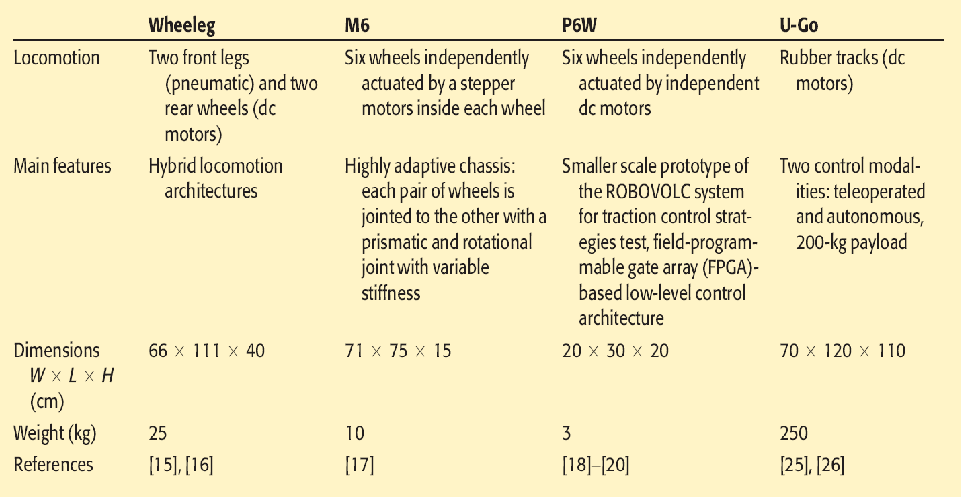
\includegraphics[scale=0.33]{figure.png}
	\caption{Table Specifications.\footnote{Image copy of ``\textit{IEEE Robotics And Automation Society}'', Volume $19$ No. $1$ March $2012$ ISSN $1070-9932$ \url{http://www.ieee-ras.org/ram}, page $44$}}
      \label{fig9}
    \end{figure}
\end{frame}


\subsection{Robot}
\begin{frame}
\frametitle{Robot}
    \begin{figure}[H]
	\centering
      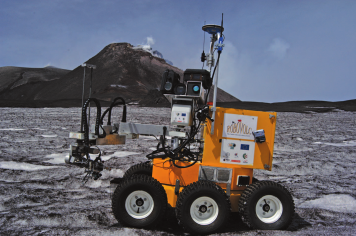
\includegraphics[scale=0.9]{robovolc.png}
	\caption{ROBOVOLC in action on top of Mt. Etna.\footnote{Image copy of ``\textit{IEEE Robotics And Automation Society}'', Volume $19$ No. $1$ March $2012$ ISSN $1070-9932$ \url{http://www.ieee-ras.org/ram}, page $45$}}
      \label{fig9}
    \end{figure}
\end{frame}

\begin{frame}
    \begin{figure}[H]
	\centering
      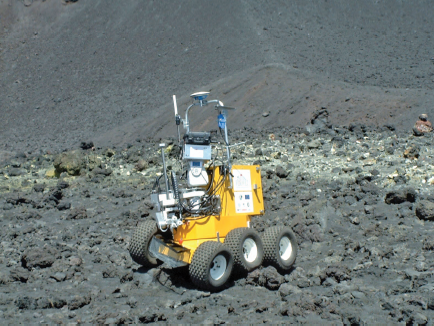
\includegraphics[scale=0.5]{8.png}
	\caption{ROBOVOLC in action on rocky terrain.\footnote{Image copy of ``\textit{IEEE Robotics And Automation Society}'', Volume $19$ No. $1$ March $2012$ ISSN $1070-9932$ \url{http://www.ieee-ras.org/ram}, page $45$}}
      \label{fig25}
    \end{figure}
\end{frame}

\subsection{The Mechanical Platform}
\begin{frame}
 \frametitle{The Mechanical Platform}
\begin{itemize}
 \item The Mechanical Platform. \pause
 \item Control Hardware Architecture. \pause
 \item Navigation and Localization System. \pause
 \item The Science Sensor Package.
\end{itemize}
\end{frame}

\subsection{Control Hardware Architecture}
\begin{frame}
 \frametitle{Control Hardware Architecture}
   \begin{figure}[H]
	\centering
      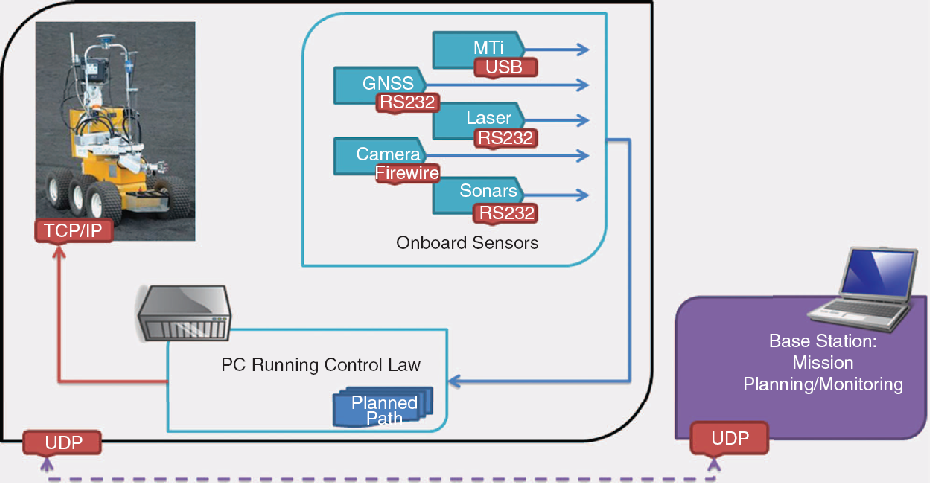
\includegraphics[scale=0.343]{plain.png}
	\caption{Navigation System Control Architecture.\footnote{Image copy of ``\textit{IEEE Robotics And Automation Society}'', Volume $19$ No. $1$ March $2012$ ISSN $1070-9932$ \url{http://www.ieee-ras.org/ram}, page $46$}}
      \label{fig25}
    \end{figure}
\end{frame}

\subsection{The Science Sensor Package}
\begin{frame}
 \frametitle{The Science Sensor Package}
\begin{figure}[H]
	\centering
      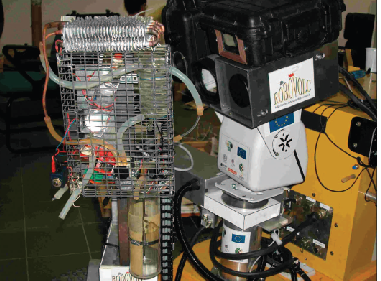
\includegraphics[scale=0.58]{9.png}
	\caption{\scriptsize The gas sampling system on the left and the pan-tilt turret on the right.\footnote{Image copy of ``\textit{IEEE Robotics And Automation Society}'', Volume $19$ No. $1$ March $2012$ ISSN $1070-9932$ \url{http://www.ieee-ras.org/ram}, page $46$}}
      \label{fig25}
    \end{figure}
\end{frame}

\begin{frame}
\begin{figure}[H]
	\centering
      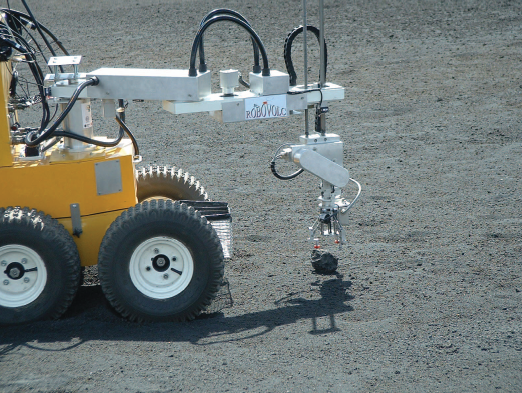
\includegraphics[scale=0.45]{10.png}
	\caption{Rock sampling with the ROBOVOLC manipulator.\footnote{Image copy of ``\textit{IEEE Robotics And Automation Society}'', Volume $19$ No. $1$ March $2012$ ISSN $1070-9932$ \url{http://www.ieee-ras.org/ram}, page $47$}}
      \label{fig25}
    \end{figure}
\end{frame}

\section{Results}
\subsection{Scientific Data Collected}
\begin{frame}
\frametitle{Scientific Data Collected}
  \begin{itemize}
   \item Video Camera Images. \pause
   \item Infrared Camera Images. \pause
   \item DGPS Data. \pause
   \item Still-Image Camera and Stereo Images. \pause
   \item Gas Sampling and Analysis. \pause
   \item Doppler Radar. \pause
   \item Rock Collecting.
  \end{itemize}
\end{frame}

\subsection{Video Camera Images}
\begin{frame}
\frametitle{Video Camera Images}
  \begin{figure}[H]
	\centering
		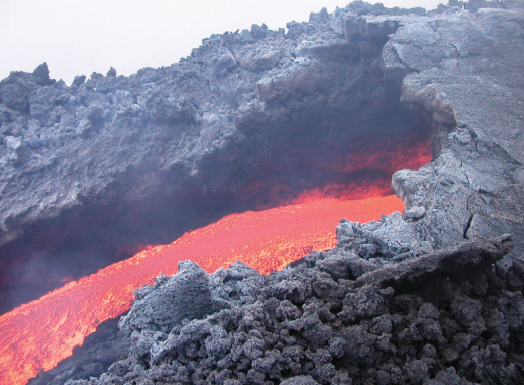
\includegraphics[scale=0.43]{image1.png}
	\caption{Example image of hot lava flow \footnote{Image copy of ``\textit{IEEE Robotics And Automation Society}'', Volume $19$ No. $1$ March $2012$ ISSN $1070-9932$ \url{http://www.ieee-ras.org/ram}, page $47$}}
	\label{fig1}
\end{figure}
\end{frame}

\subsection{Infrared Camera Images}
\begin{frame}
\frametitle{Infrared Camera Images}
  \begin{figure}[H]
	\centering
		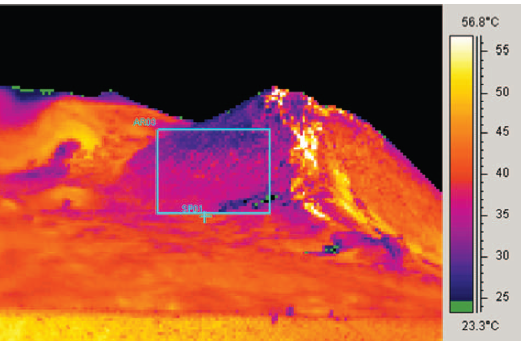
\includegraphics[scale=0.48]{infra.png}
	\caption{Example Crater viewed form the IR camera \footnote{Image copy of ``\textit{IEEE Robotics And Automation Society}'', Volume $19$ No. $1$ March $2012$ ISSN $1070-9932$ \url{http://www.ieee-ras.org/ram}, page $48$}}
	\label{fig2}
\end{figure}
\end{frame}

\section{Conclusions}
\begin{frame}
    \frametitle{Conclusions}
      \begin{itemize}
       \item The adoption of robotics in volcanology is still in its infancy, since only few prototypes have been realized, and most of the research activity needs further investigation and resources. Despite this, robots have shown to be quite useful for environmental measurements and, in general, for taking measurements in dangerous locations. \pause
       \item The performed research activity in the development of robots for volcanic measurement and exploration allowed us to better understand and solve problems related to the adoption of robots in extreme environments, as well as in other contexts such as search and rescue along with operations in other hazardous situations and areas.
      \end{itemize}
\end{frame}

\begin{frame}
\frametitle{Conclusions}
\begin{itemize}
 \item They believe that robots used to obtain scientific data will help to further increase the quality and quantity of information needed for a clearer understanding of volcanoes and also serve to reduce risks for volcanologists. \pause
 \item The Volcan UAV, the U-Go robot, and the ROBOVOLC system are maintained operative and are now useful tools for the volcanologists of INGV, being used each year in several missions, both to perform measurements and to further develop robotic strategies.
\end{itemize}
\end{frame}

\section{Bibliography}
\begin{frame}
\frametitle{Bibliography}
\begin{thebibliography}{10}
\bibitem{page1} \textit{IEEE ROBOTICS AND AUTOMATION SOCIETY Volume 19}, No. 1 March 2012 ISSN 1070-9932 \url{http://www.ieee-ras.org/ram}.

\bibitem{article} \textbf{Article:} Volcanic Environments Robots for exploration and Measurement
 By G. Muscato, F. Bonaccorso, L. Cantelli, D. Longo, and C.D. Melita.
\end{thebibliography}
\end{frame} 
\end{document}